\section{Introduction}

We must start out by defining \textit{entropy}.
Entropy is kind of a fancy word for uncertainty.
My past encounters with the word entropy have been mostly confusing, verging on mystical.
I'm sure many of us have been told, ``the entropy of the universe is always increasing.''
Let's leave entropy's existential baggage behind and treat it just like any other run-of-the-mill word.
The best way to get a practical feel for entropy is with an example.

We have a coin.
The coin has a red side and a grey side.
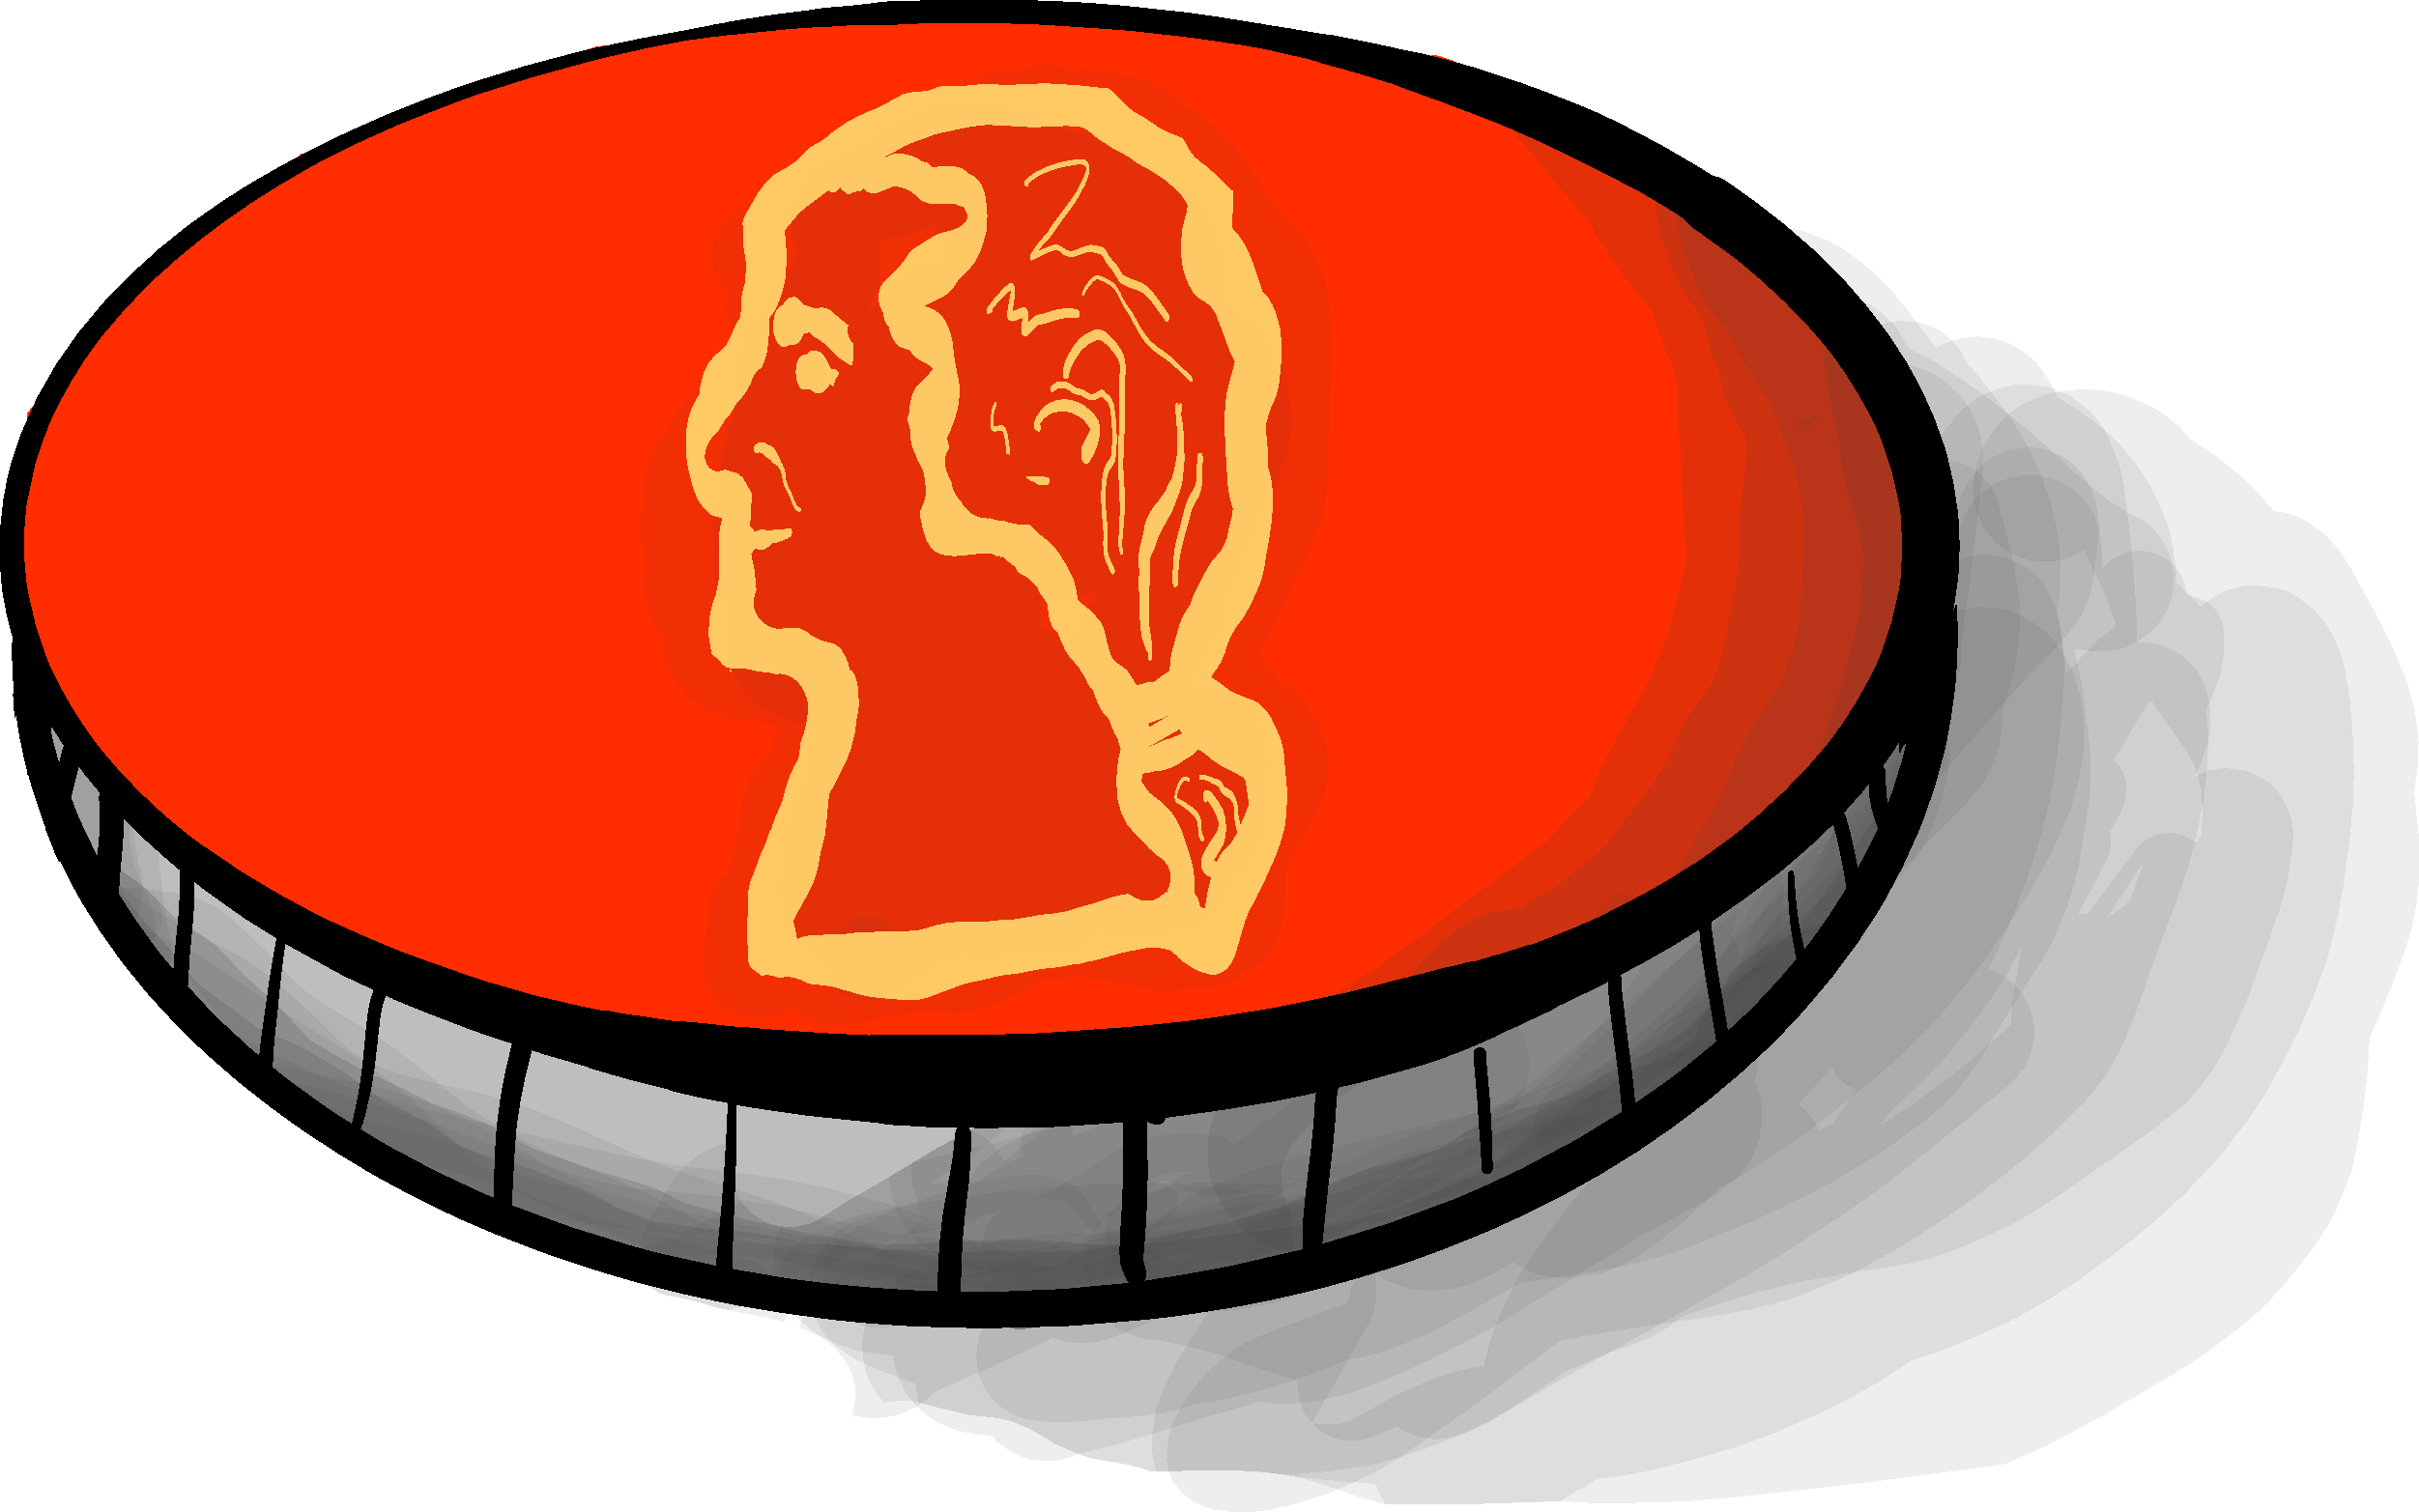
\includegraphics[width=0.3\textwidth]{img/red-coin}
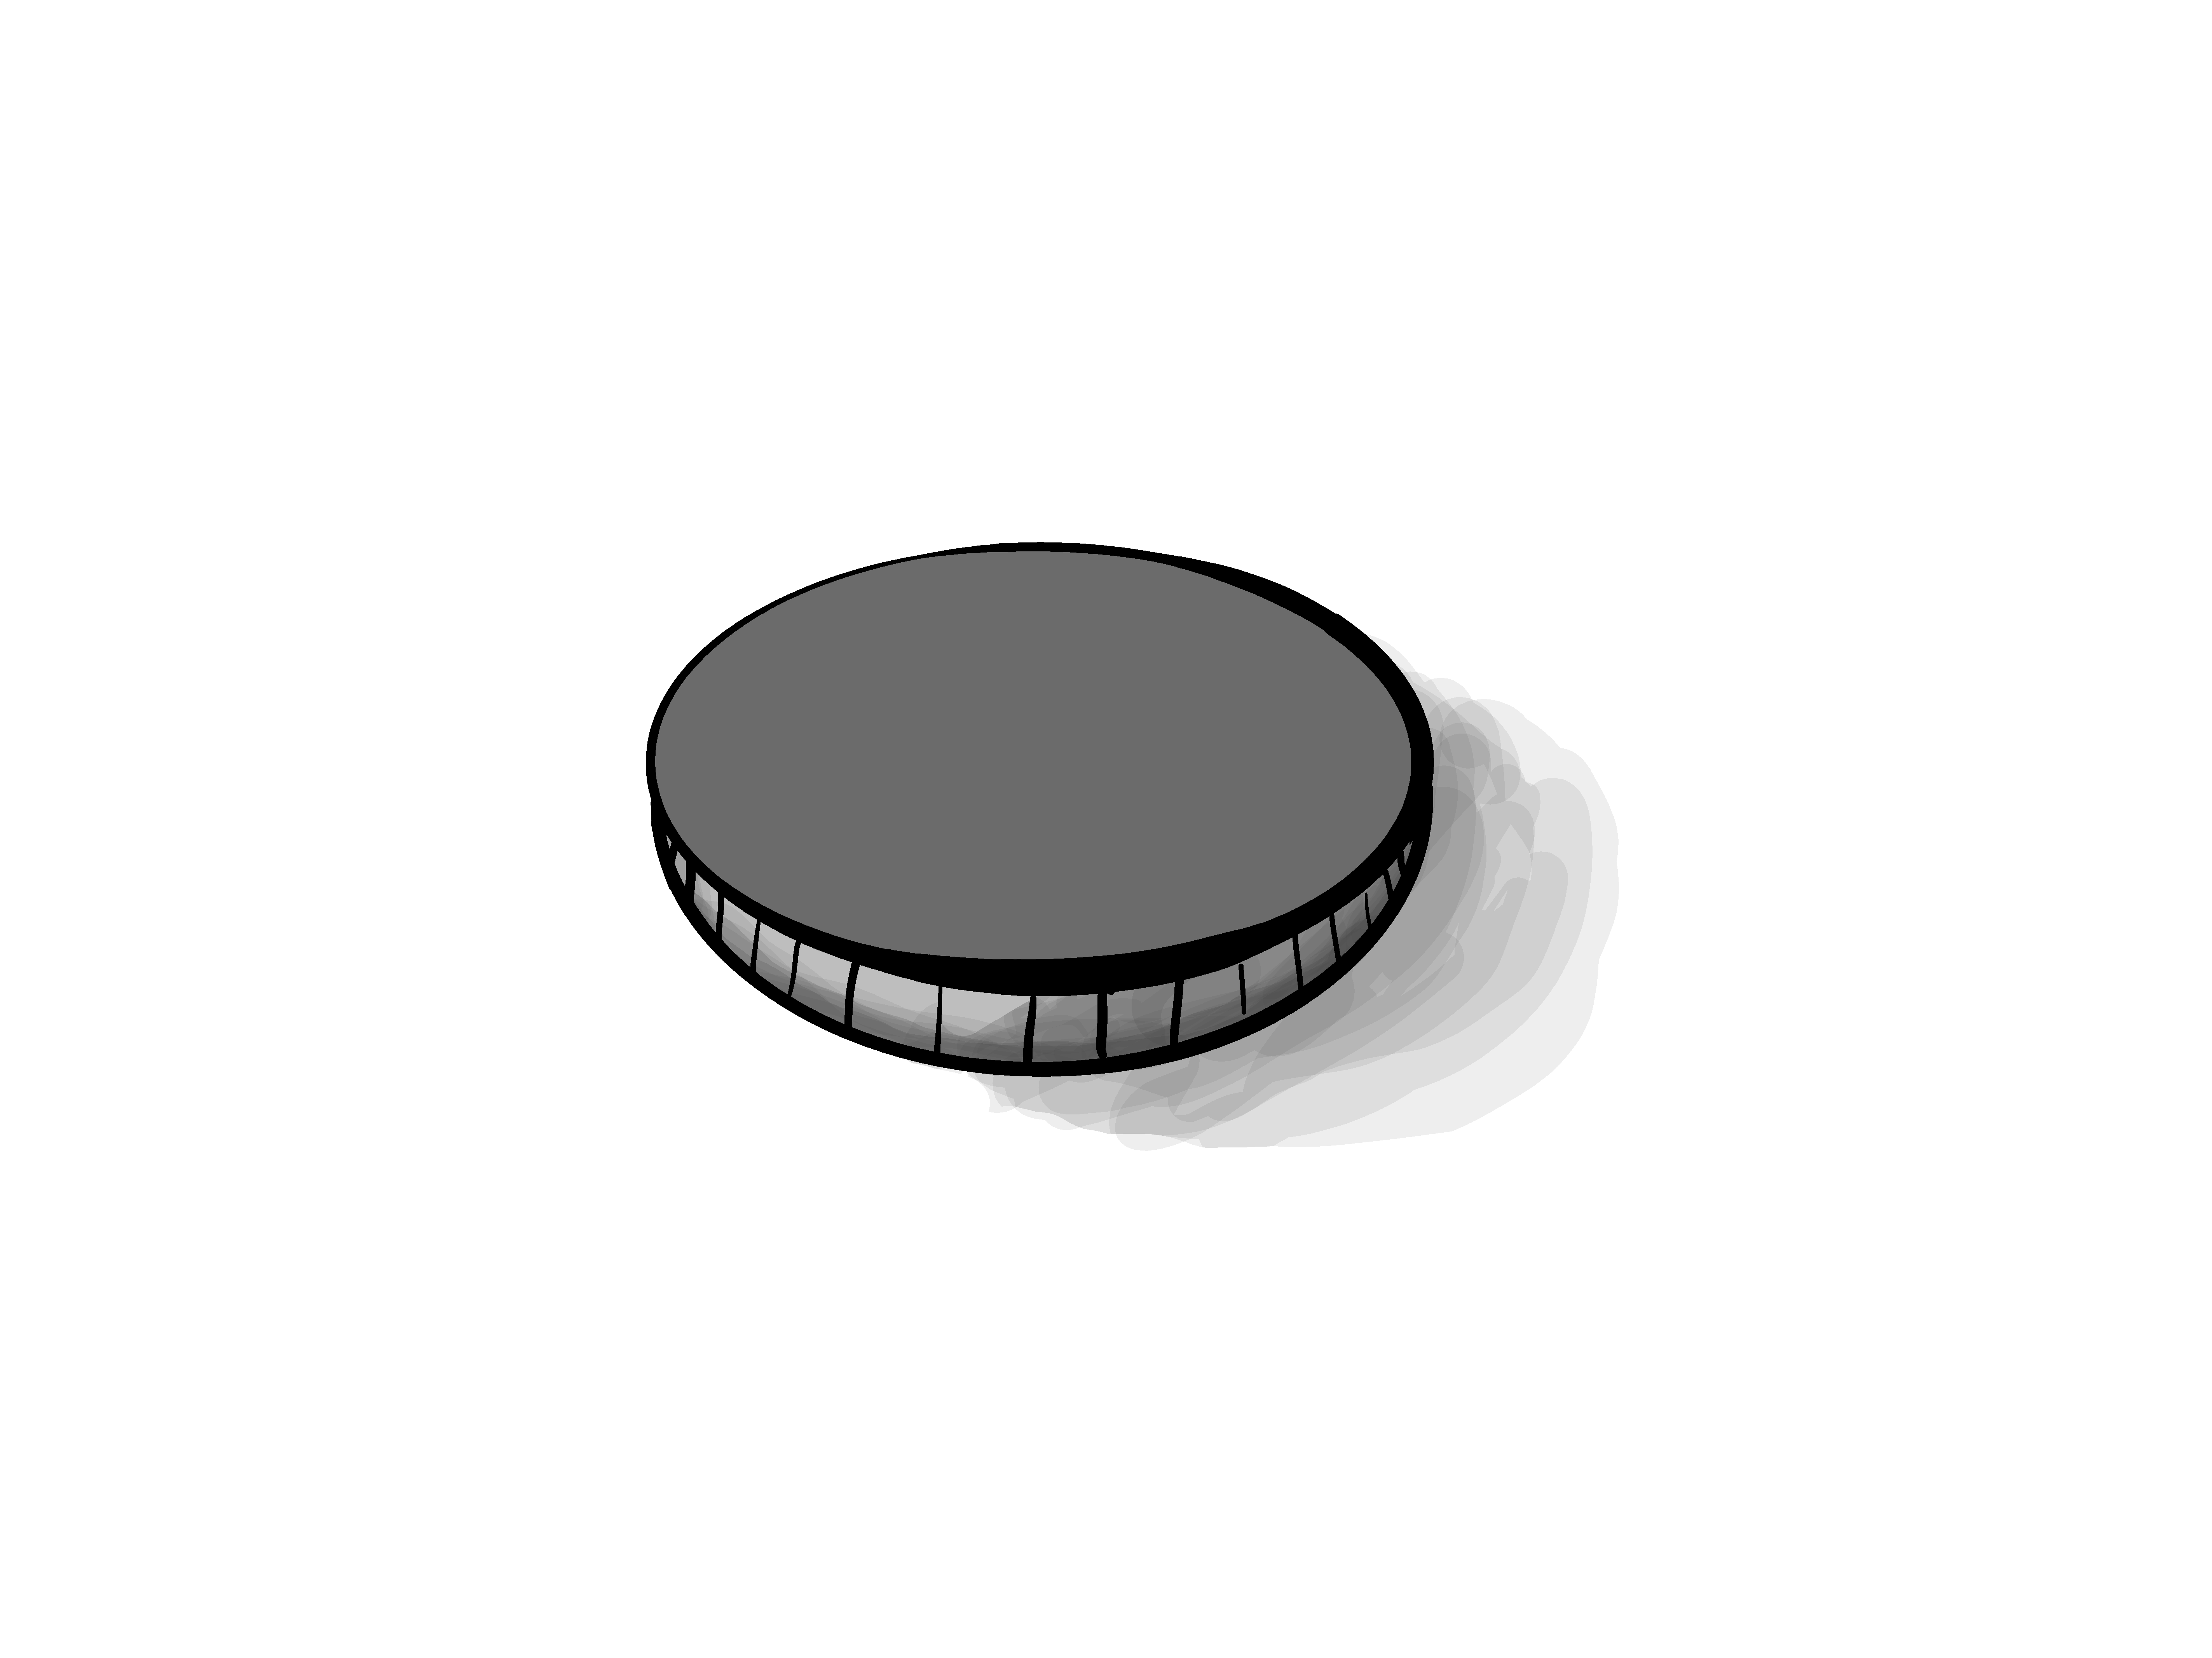
\includegraphics[width=0.3\textwidth]{img/grey-coin}
The coin is evenly weighted so if we were to throw it in the air, half of the time it would land red side up and the other half of the time it would land grey side up.
If we model our coin as a random variable $\bm{C}$, we can write this mathematically as $p(\bm{C} = \text{red}) = 0.5$ and $p(\bm{C} = \text{grey}) = 0.5$.

Let's put the coin in a box.
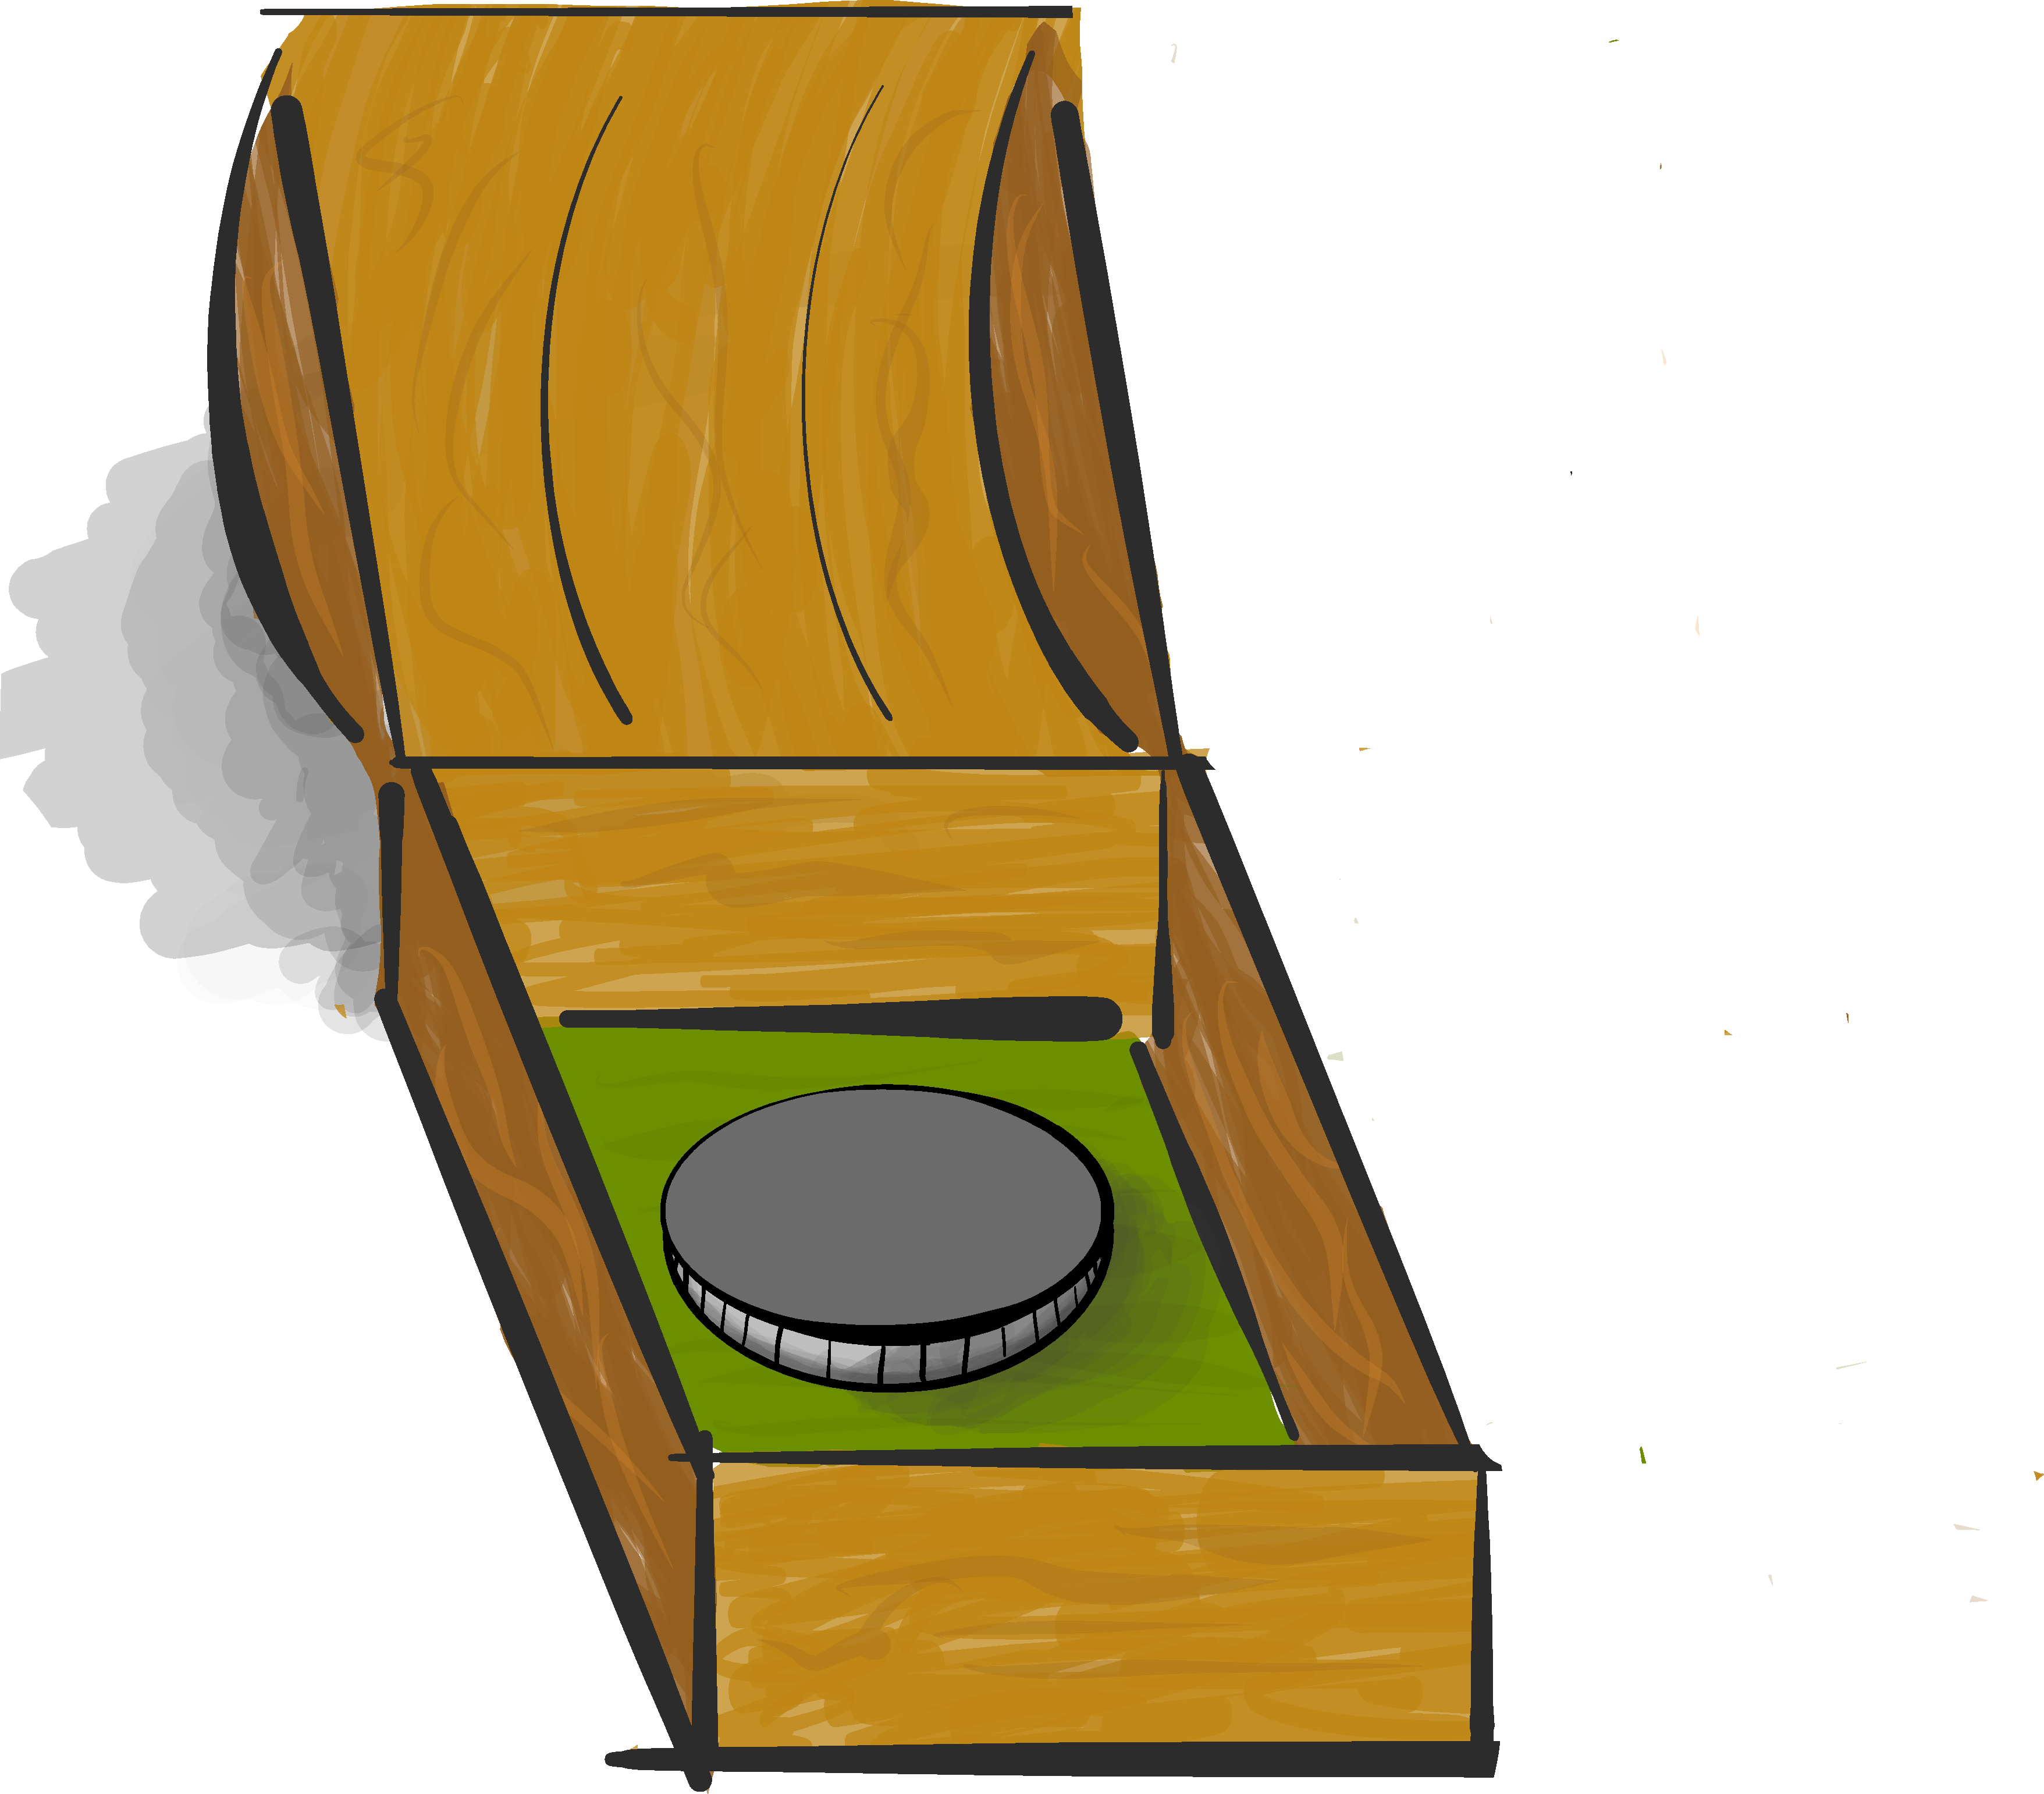
\includegraphics[width=0.3\textwidth]{img/big-box-open-coin}

Right now, the grey side of the coin is facing up.
How much uncertainty do we have in regard to the position of the coin?
None.
We know the grey side of the coin is facing up.
Thus, entropy is zero.
To say this mathematically, we write $S = 0$.

What about the entropy of the molecules that make up the coin?
What about the entropy of the universe?
We don't have to worry about any of that.
Entropy has no intrinsic meaning.
It's just a tool that we use to help us concretely understand a particular situation.
Right now we are just thinking about which way a coin is facing.
So, right now entropy just describes our uncertainty about which way that coin is facing.

Let's close the box and give it a good shake.
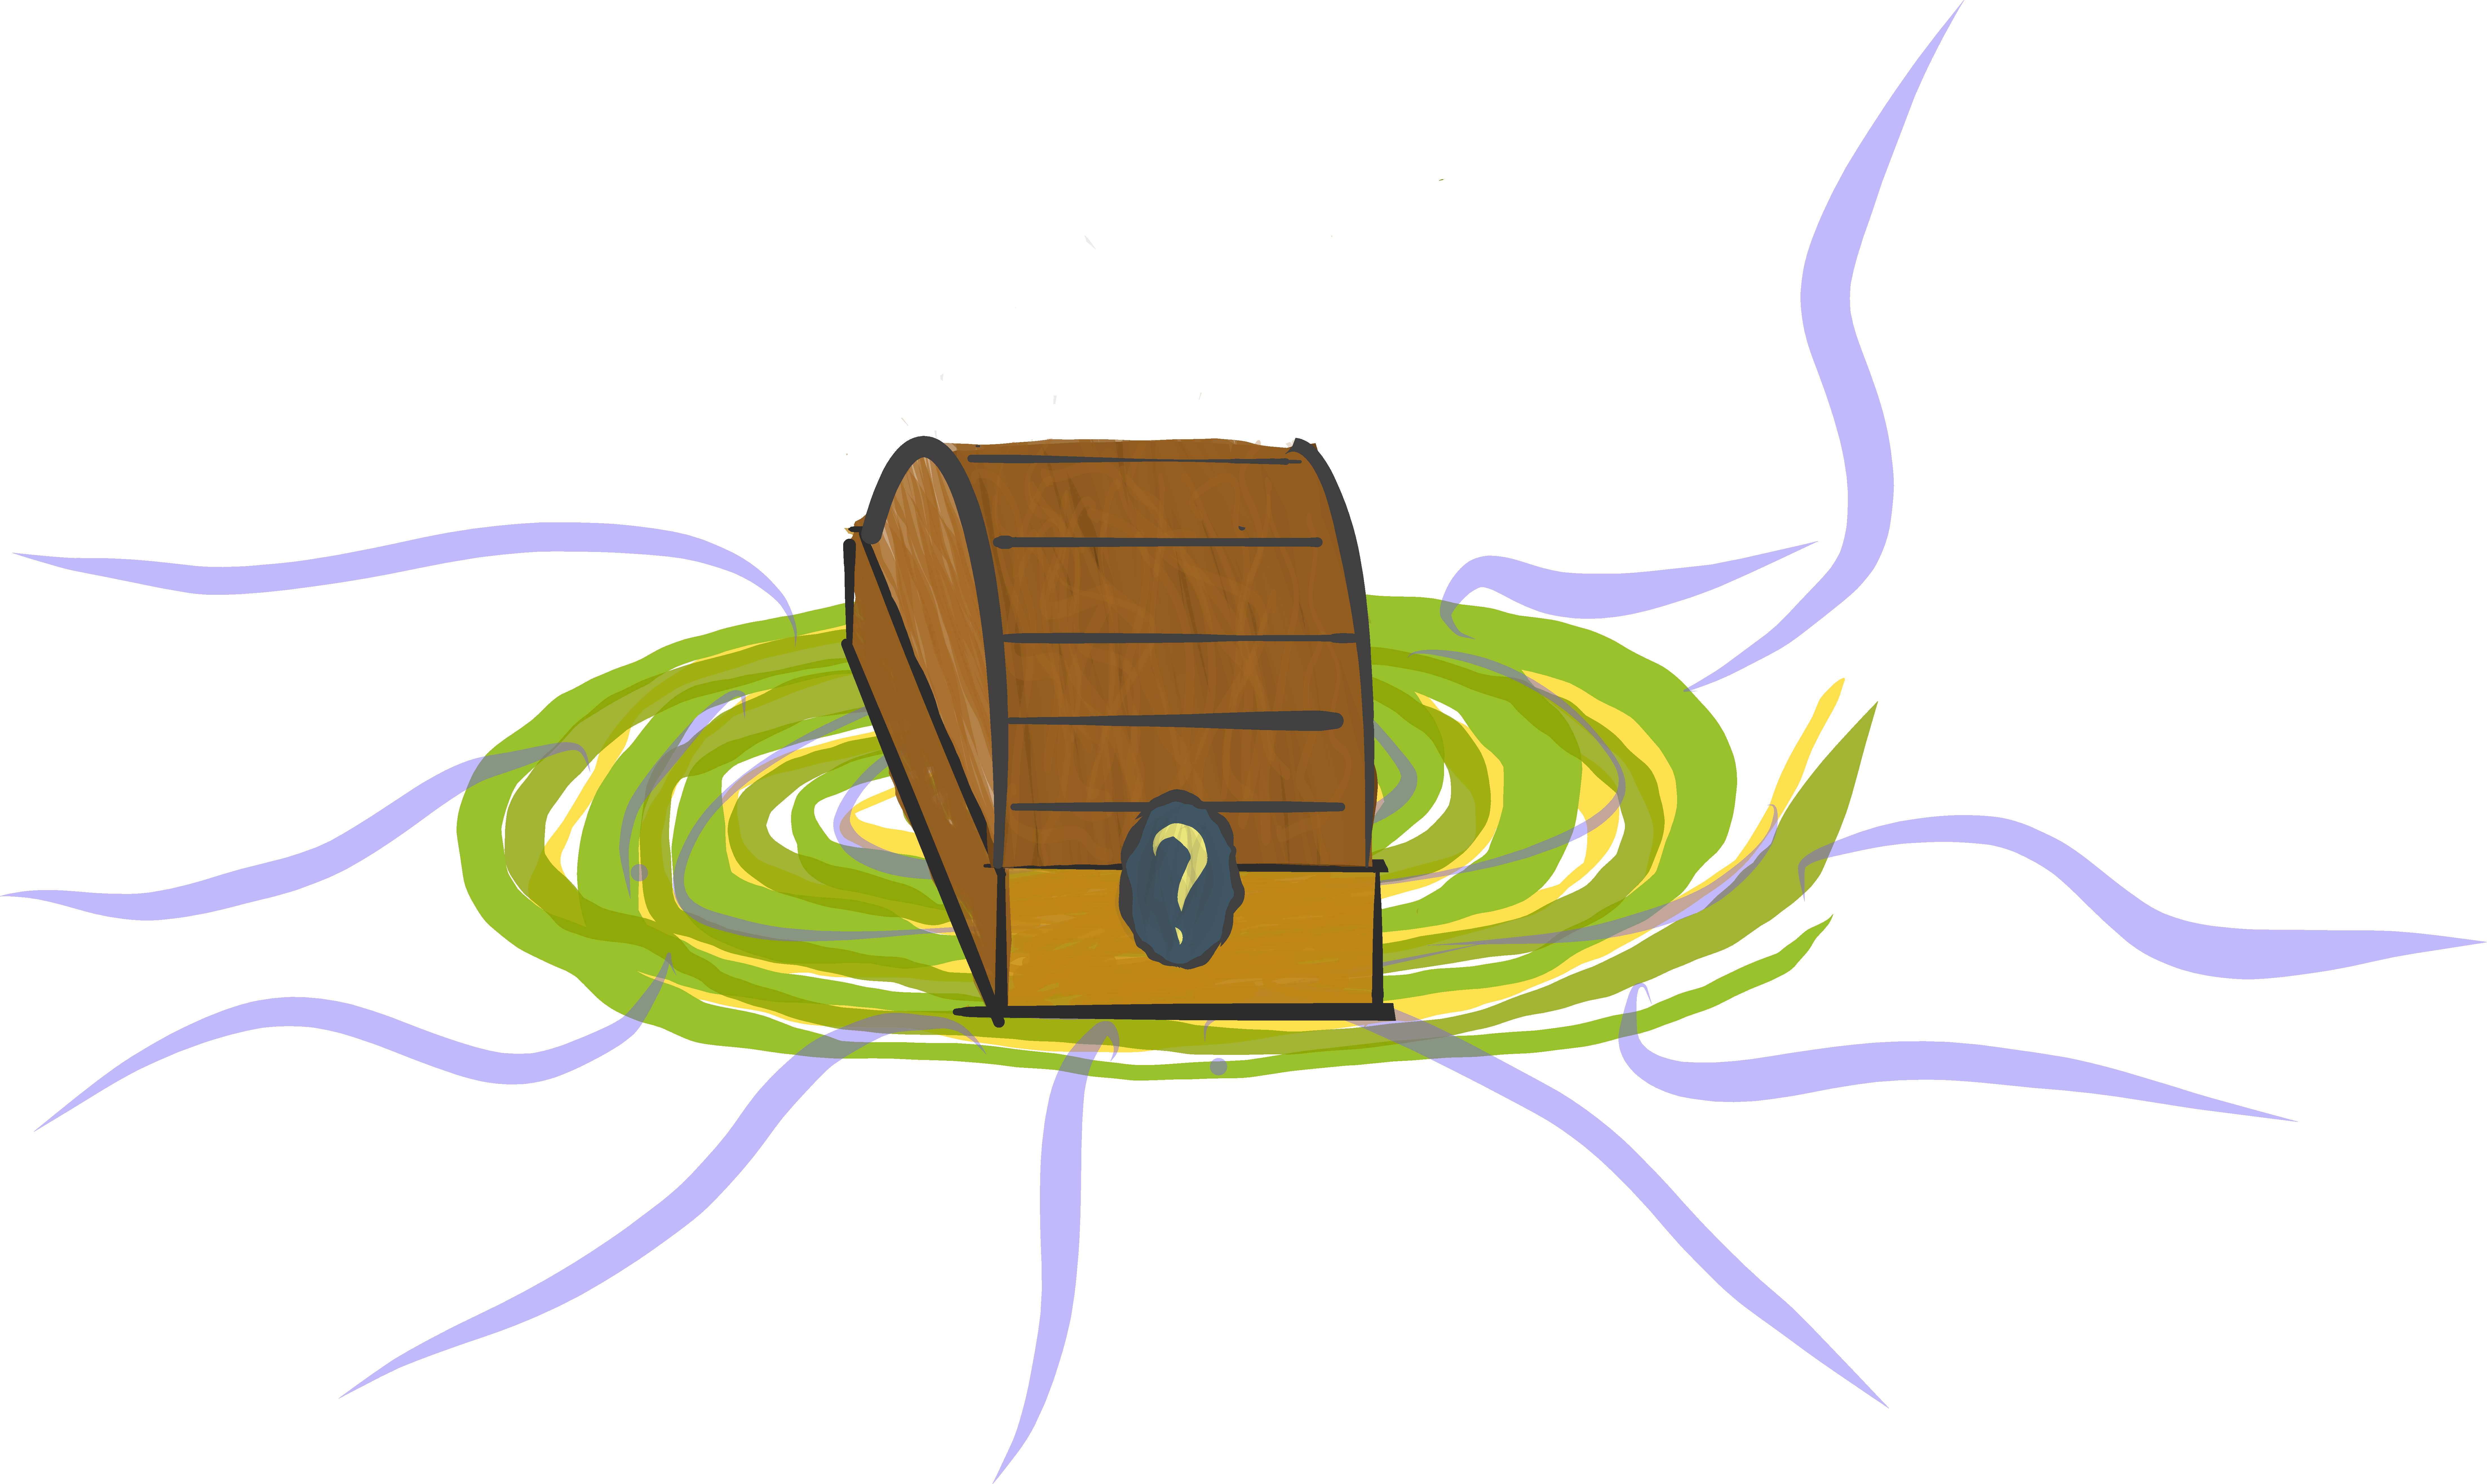
\includegraphics[width=0.3\textwidth]{img/big-box-closed-portal}
We're no longer certain of the coin's position.
So, the entropy is greater than zero, or $S > 0$.
We can use Shannon's equation to make a more specific mathematical statement about the entropy of our coin.

In general, Shannon's equation allows us to use the set of probabilities for possible outcomes from a random variable $\{p_1, p_2, \ldots, p_n\}$ to calculate the entropy of that random variable.
The equation looks like this,
\begin{align} \label{eqn:shannon}
S = \sum_{i=1}^{n} -p_i \log(p_i)
\end{align}
This equation is the main tool we'll use to work through our toy examples.
If you're curious about the intuition behind its mathematical form, check out \cite{Adami2016}.

Recall that for our coin, $\{p_{\text{red}} = 0.5, p_{\text{grey}} = 0.5 \}$.
Plugging and chugging with Equation \ref{eqn:snannon}, we calculate
\begin{align*}
S_{\text{coin}} = 1.
\end{align*}
We used the base two logarithm to perform this calculation, so the unit that describes our entropy value is the ``bit.''
For consistency's sake, we will use this unit for all the rest of the calculations we perform as well.
Thus, we say that the coin closed in the box has one bit of entropy.

Now, let's open the box and observe the state of the coin.
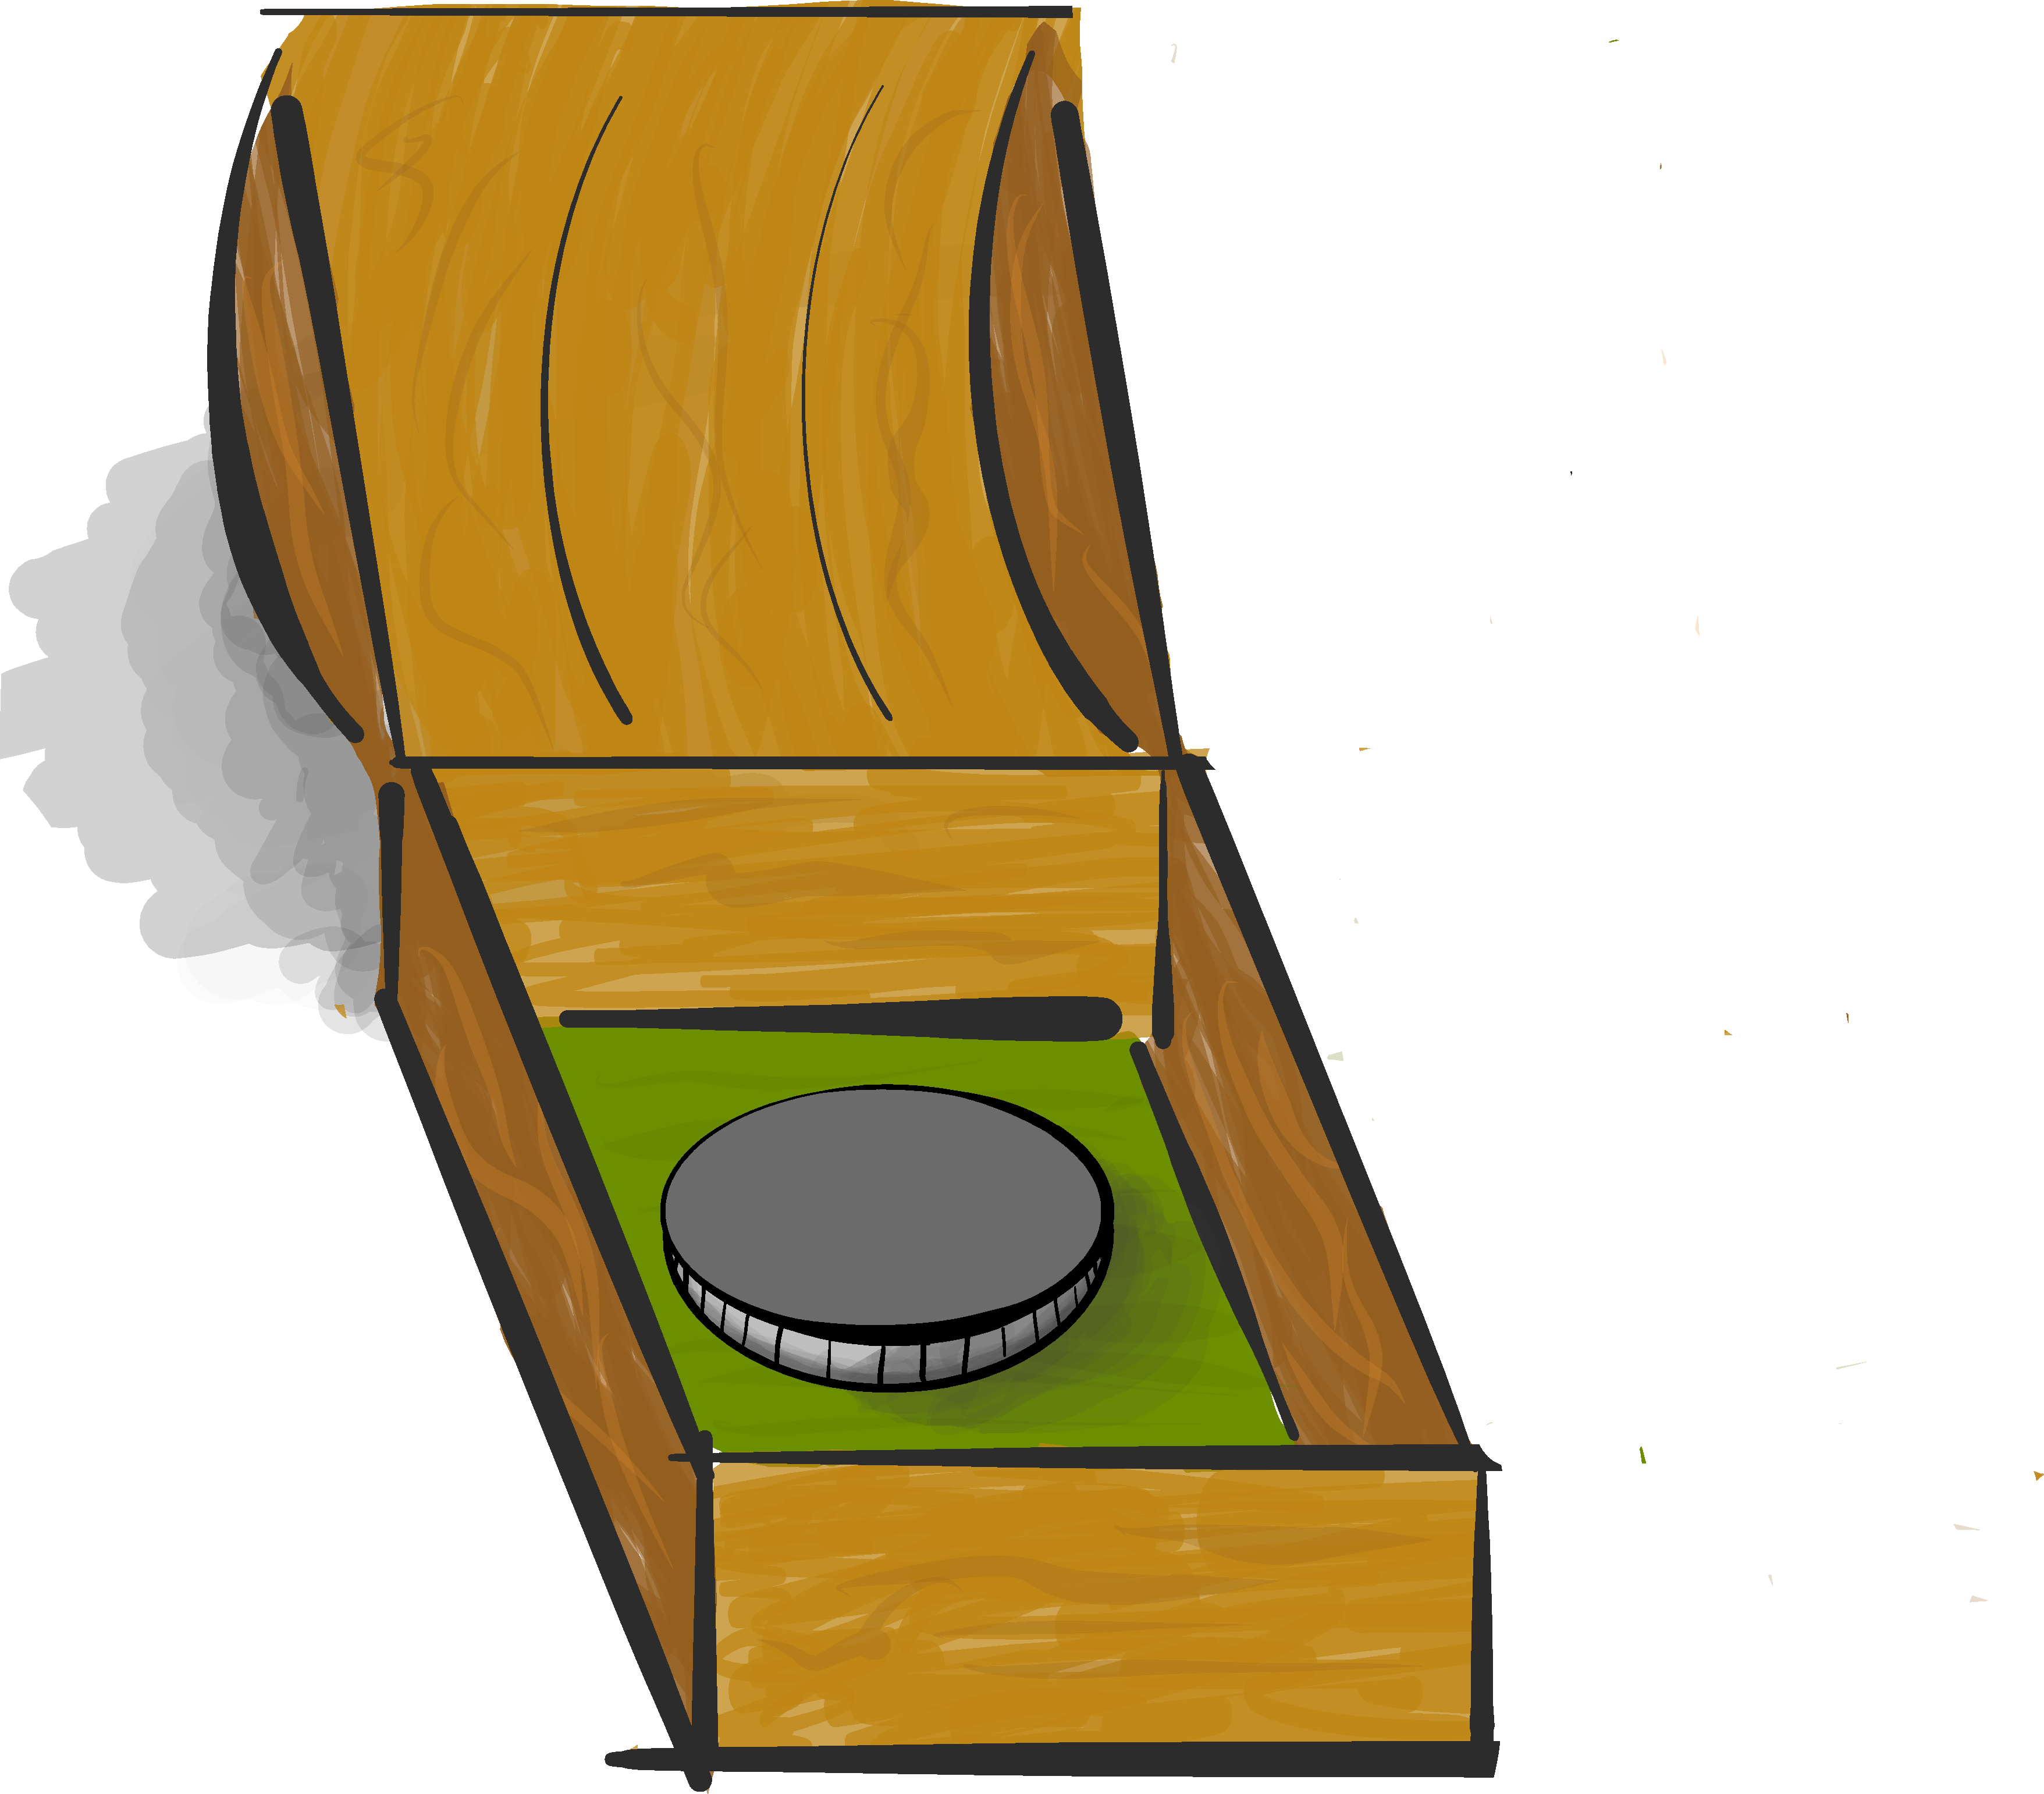
\includegraphics[width=0.3\textwidth]{img/big-box-open-coin}
We are again certain about the state of the coin, so $S = 0$.
This is where \textit{information} comes into play.
\textit{Information} is the difference between two entropies.
We can calculate the information that was gained opening the box by subtracting the ending entropy from the starting entropy,
\begin{align*}
I
&= S_{\text{before}} - S_{\text{after}} \\
&= 1 - 0 \\
&= 1
\end{align*}
We gained one bit of information.
Neat!

We can cement our intuition for what entropy measures by repeating our little thought experiment with a slightly different set up.
Now, instead of a coin we have a die.
The die has ten faces.
Nine of the faces are painted grey.
The last face is painted red.
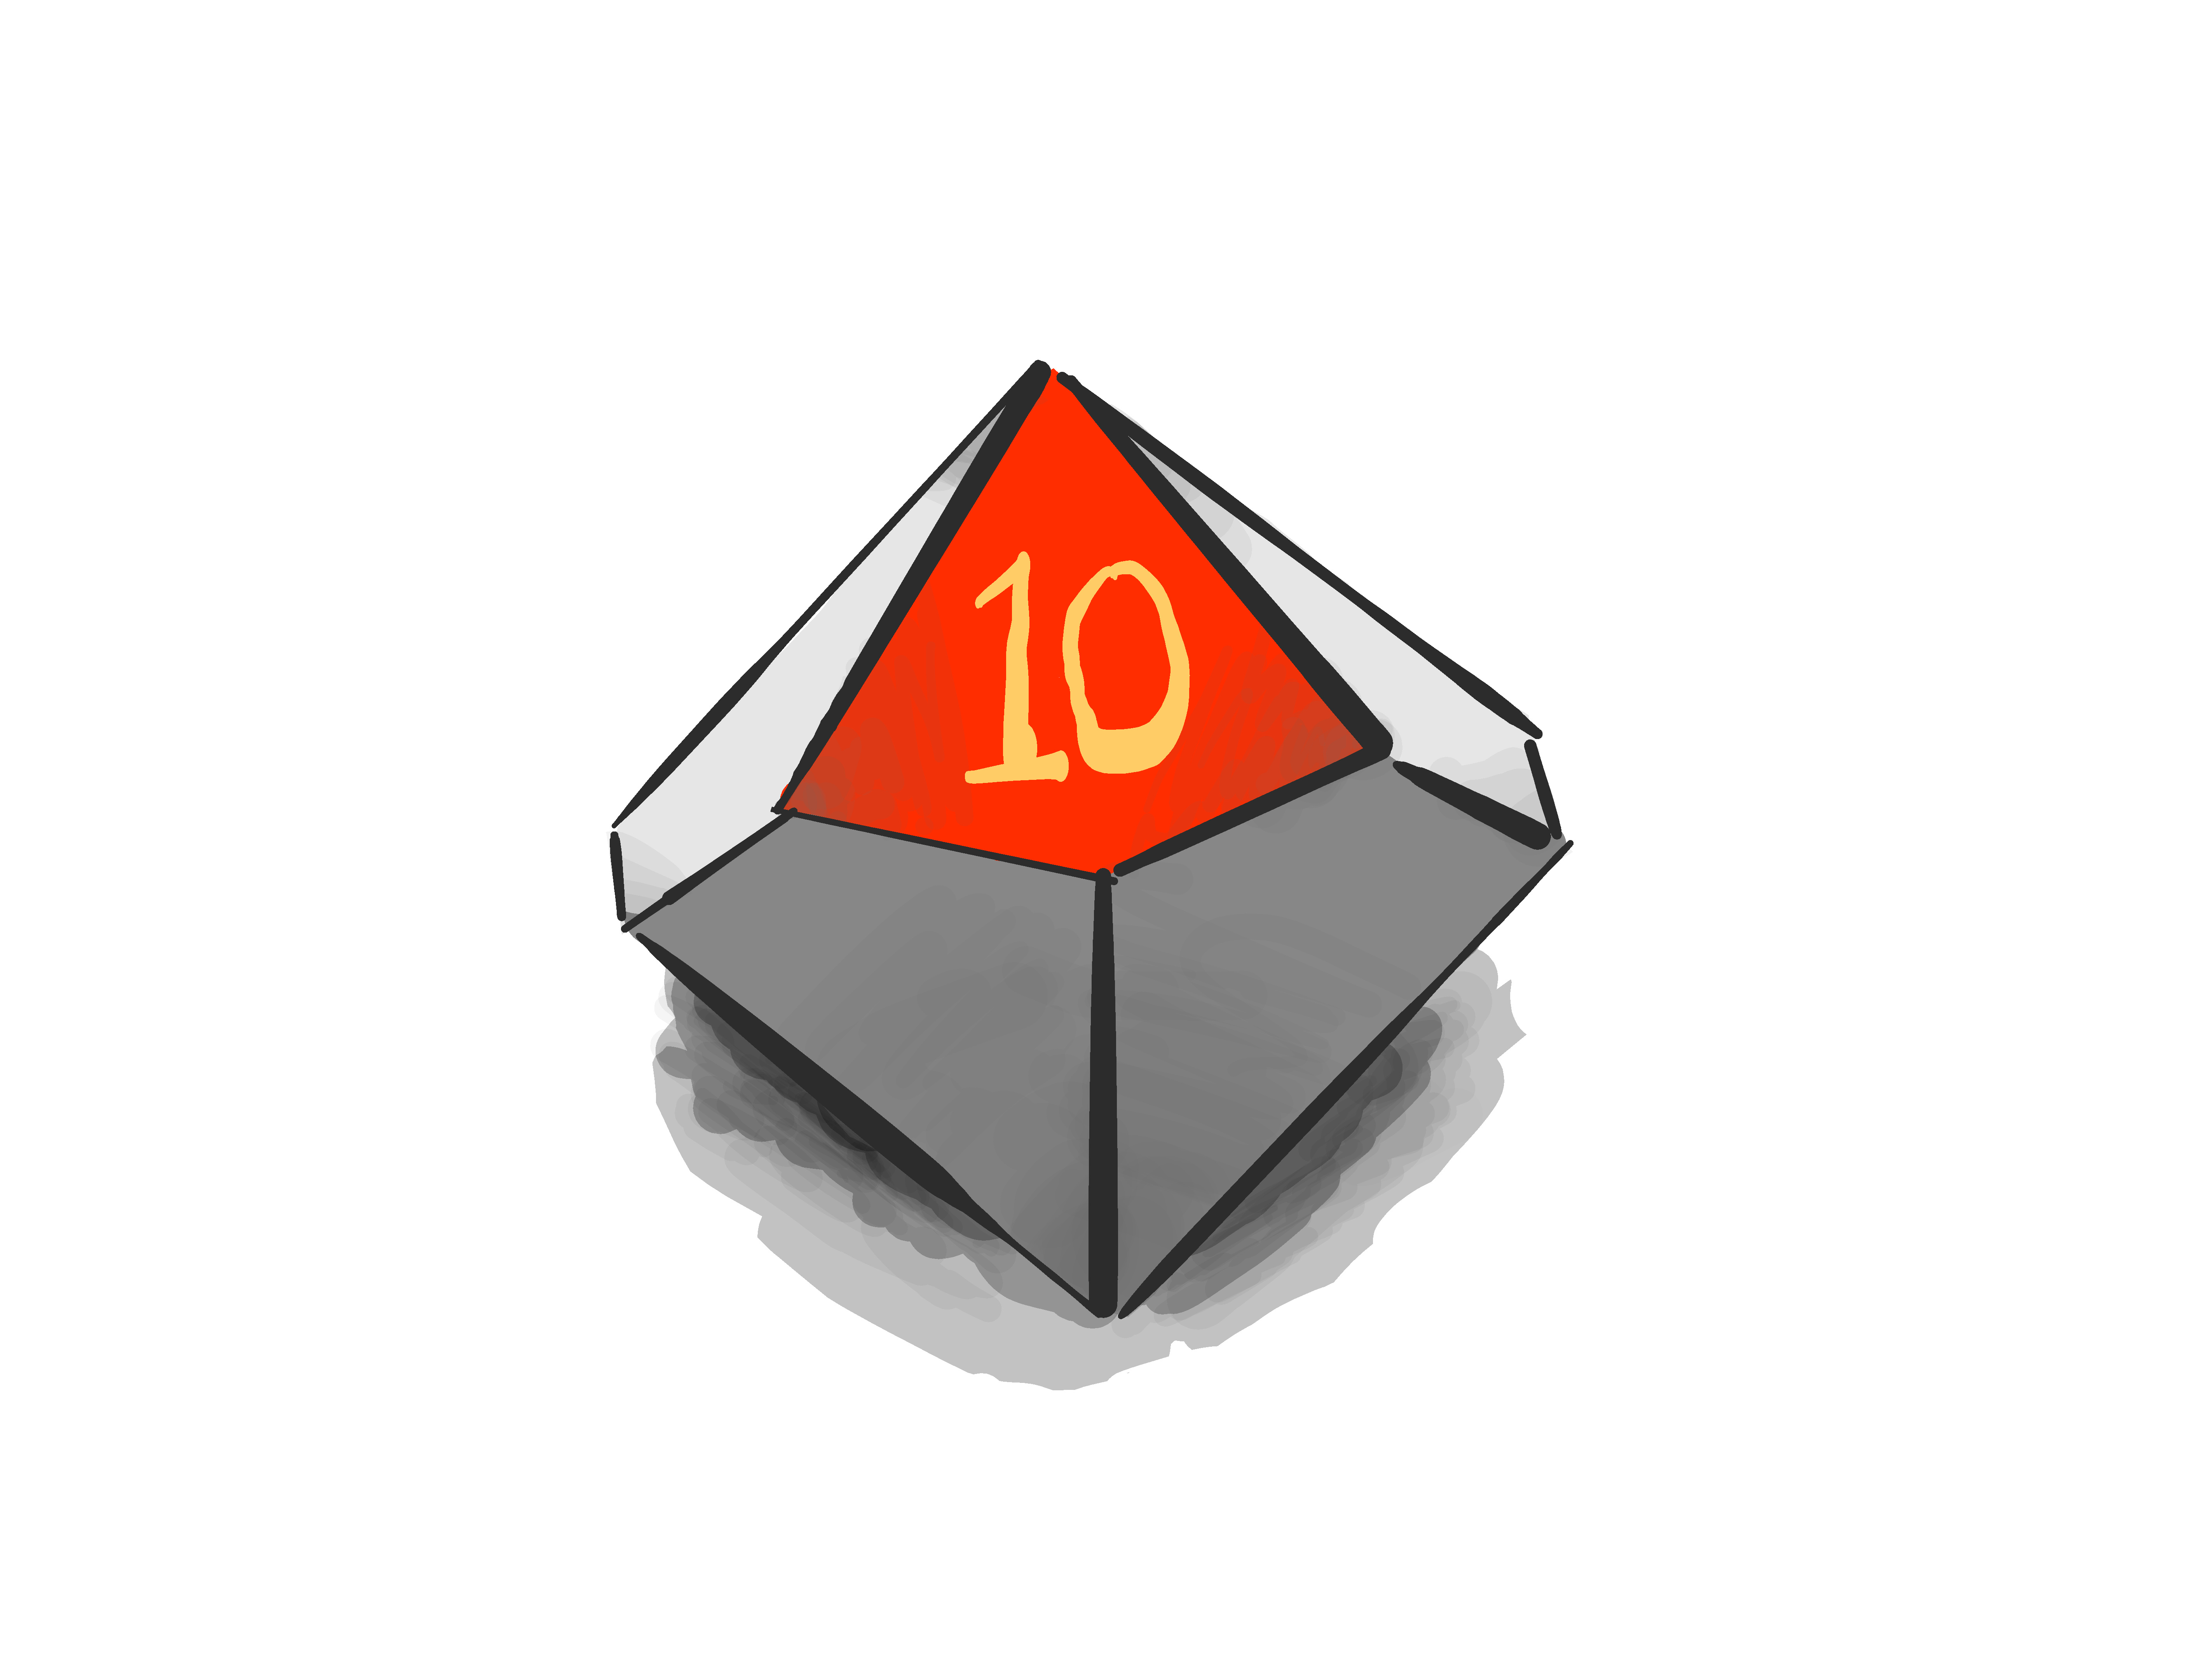
\includegraphics[width=0.3\textwidth]{img/red-die}
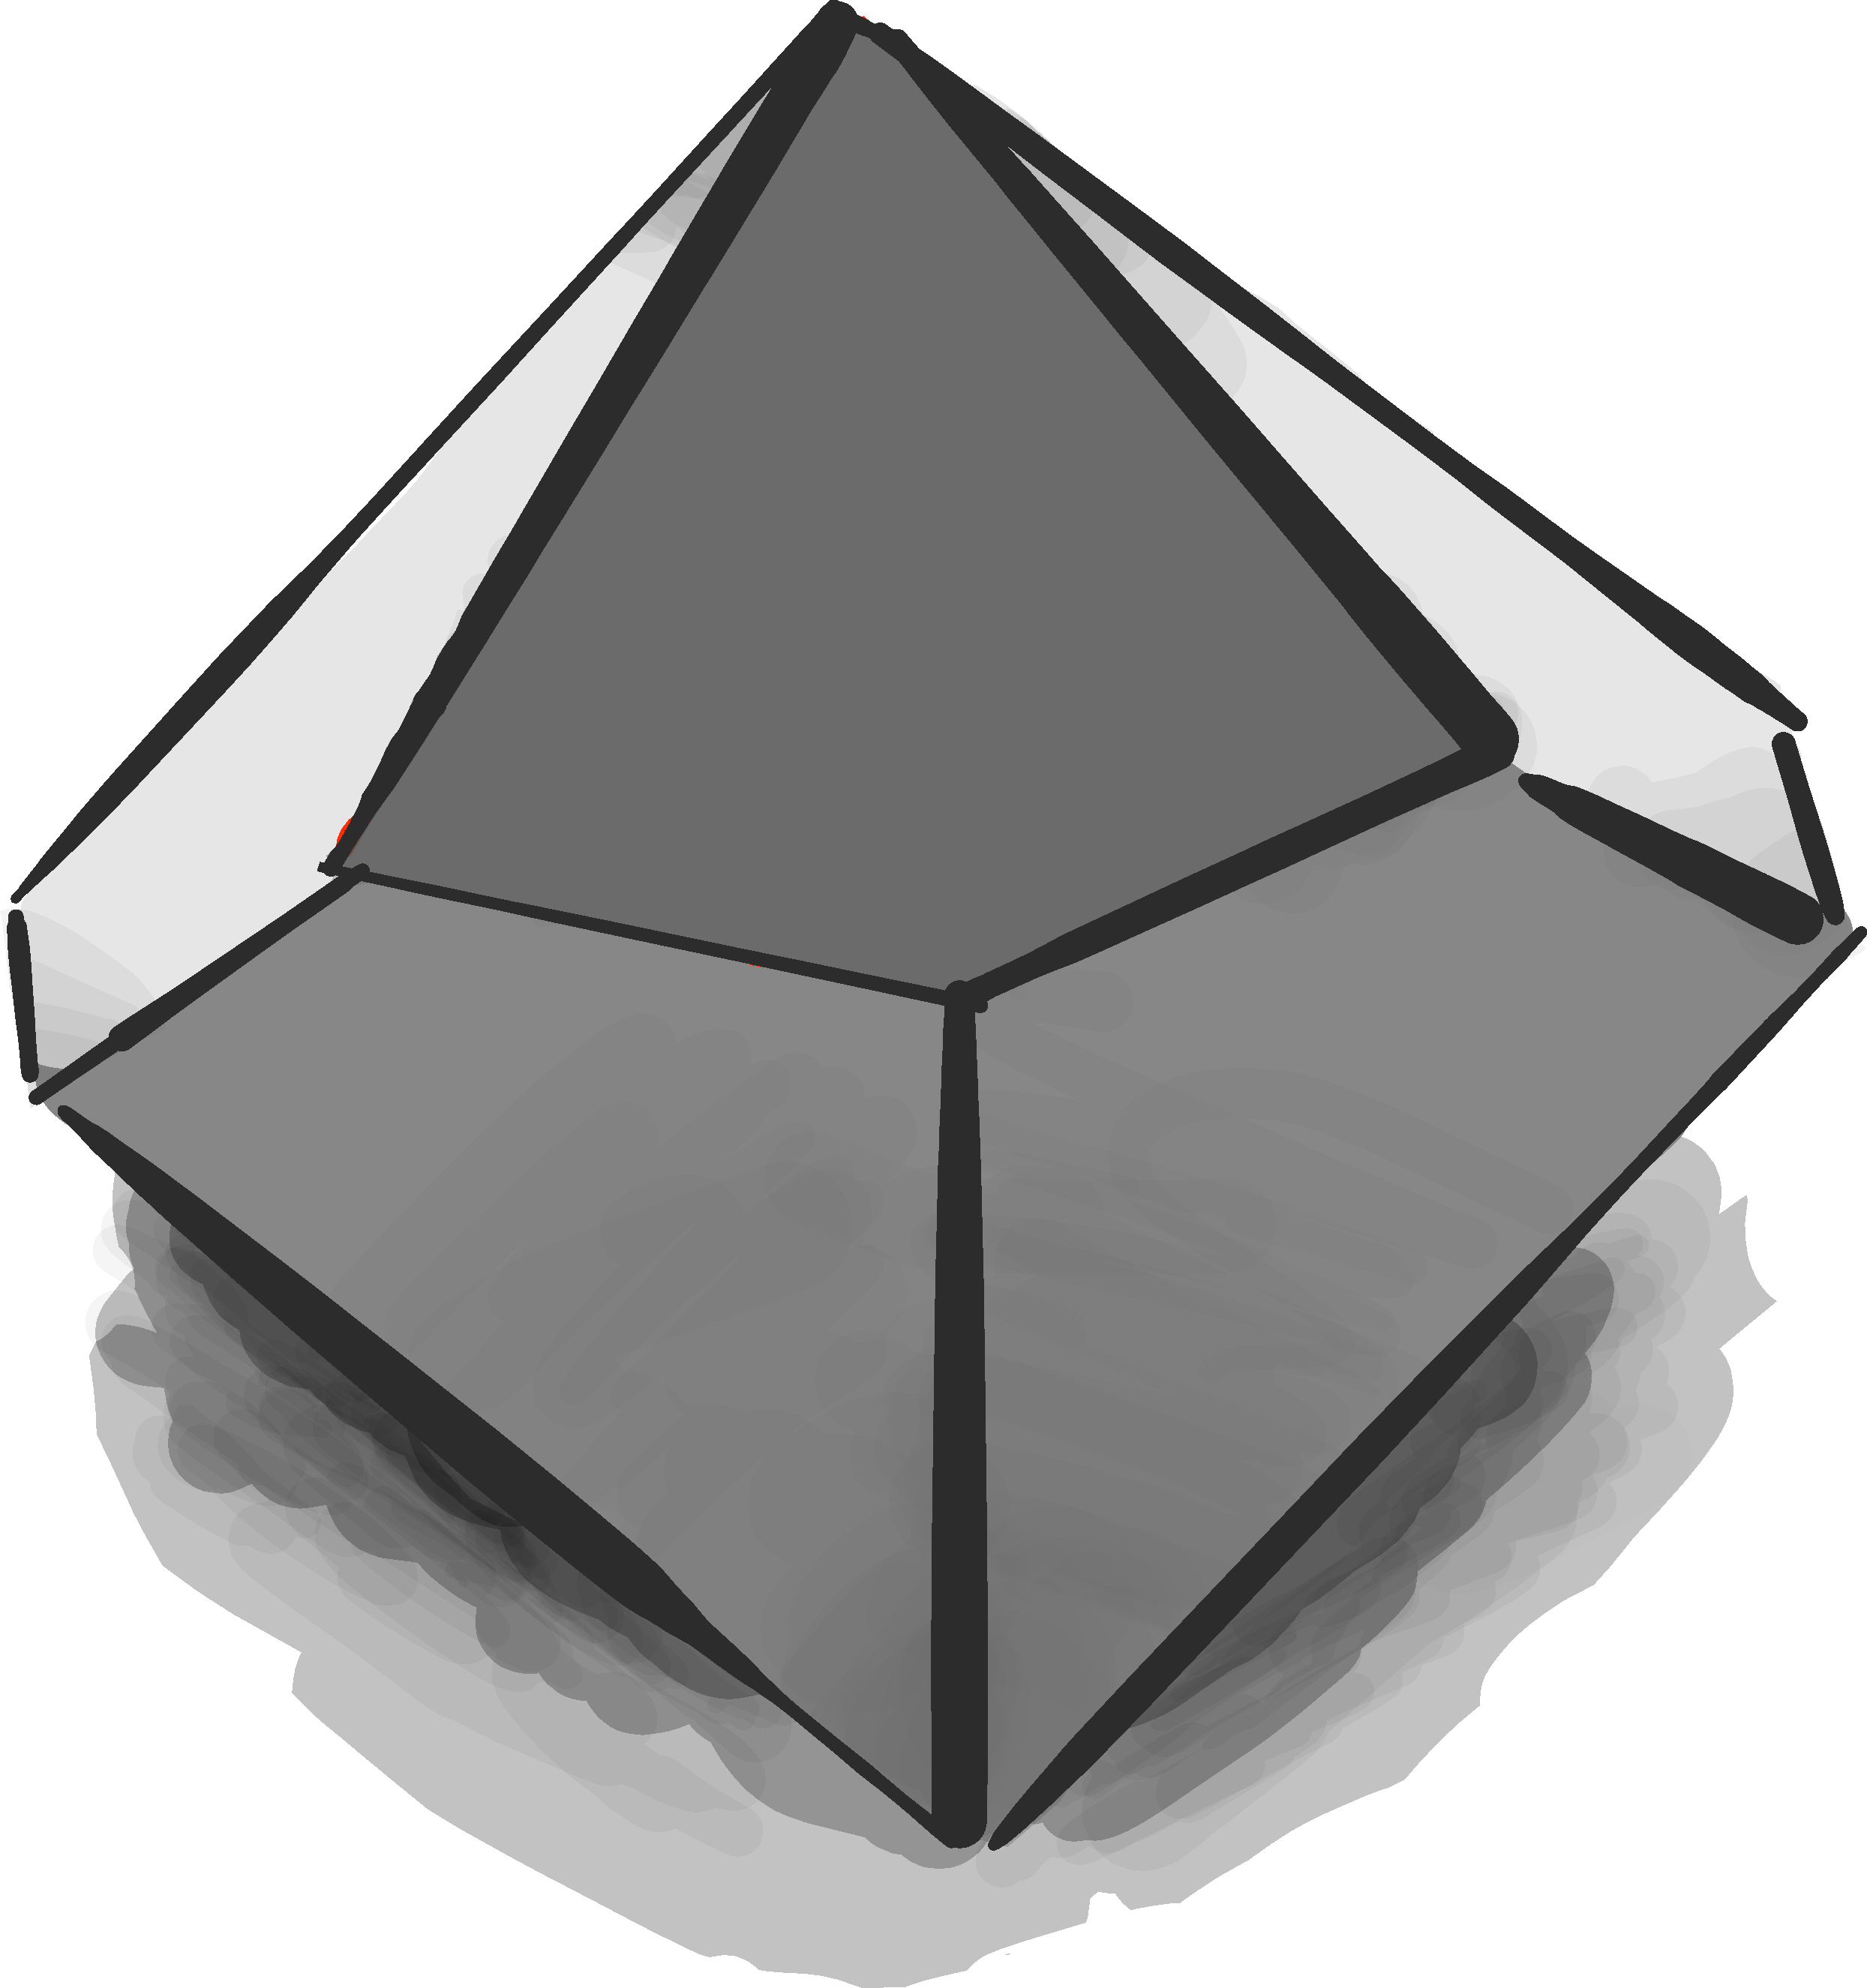
\includegraphics[width=0.3\textwidth]{img/grey-die}
The die is evenly weighted;
if we were to throw it in the air, it would land at equal frequency with any of its ten sides up.
Thus, nine times out of ten it will land with a grey side up and one time out of ten it will land with the red side up.
If we model our die as a random variable $\bm{D}$, we can write this mathematically as $p(\bm{D} = \text{red}) = 0.1$ and $p(\bm{D} = \text{grey}) = 0.9$.

Let's put the die in a box, like so.
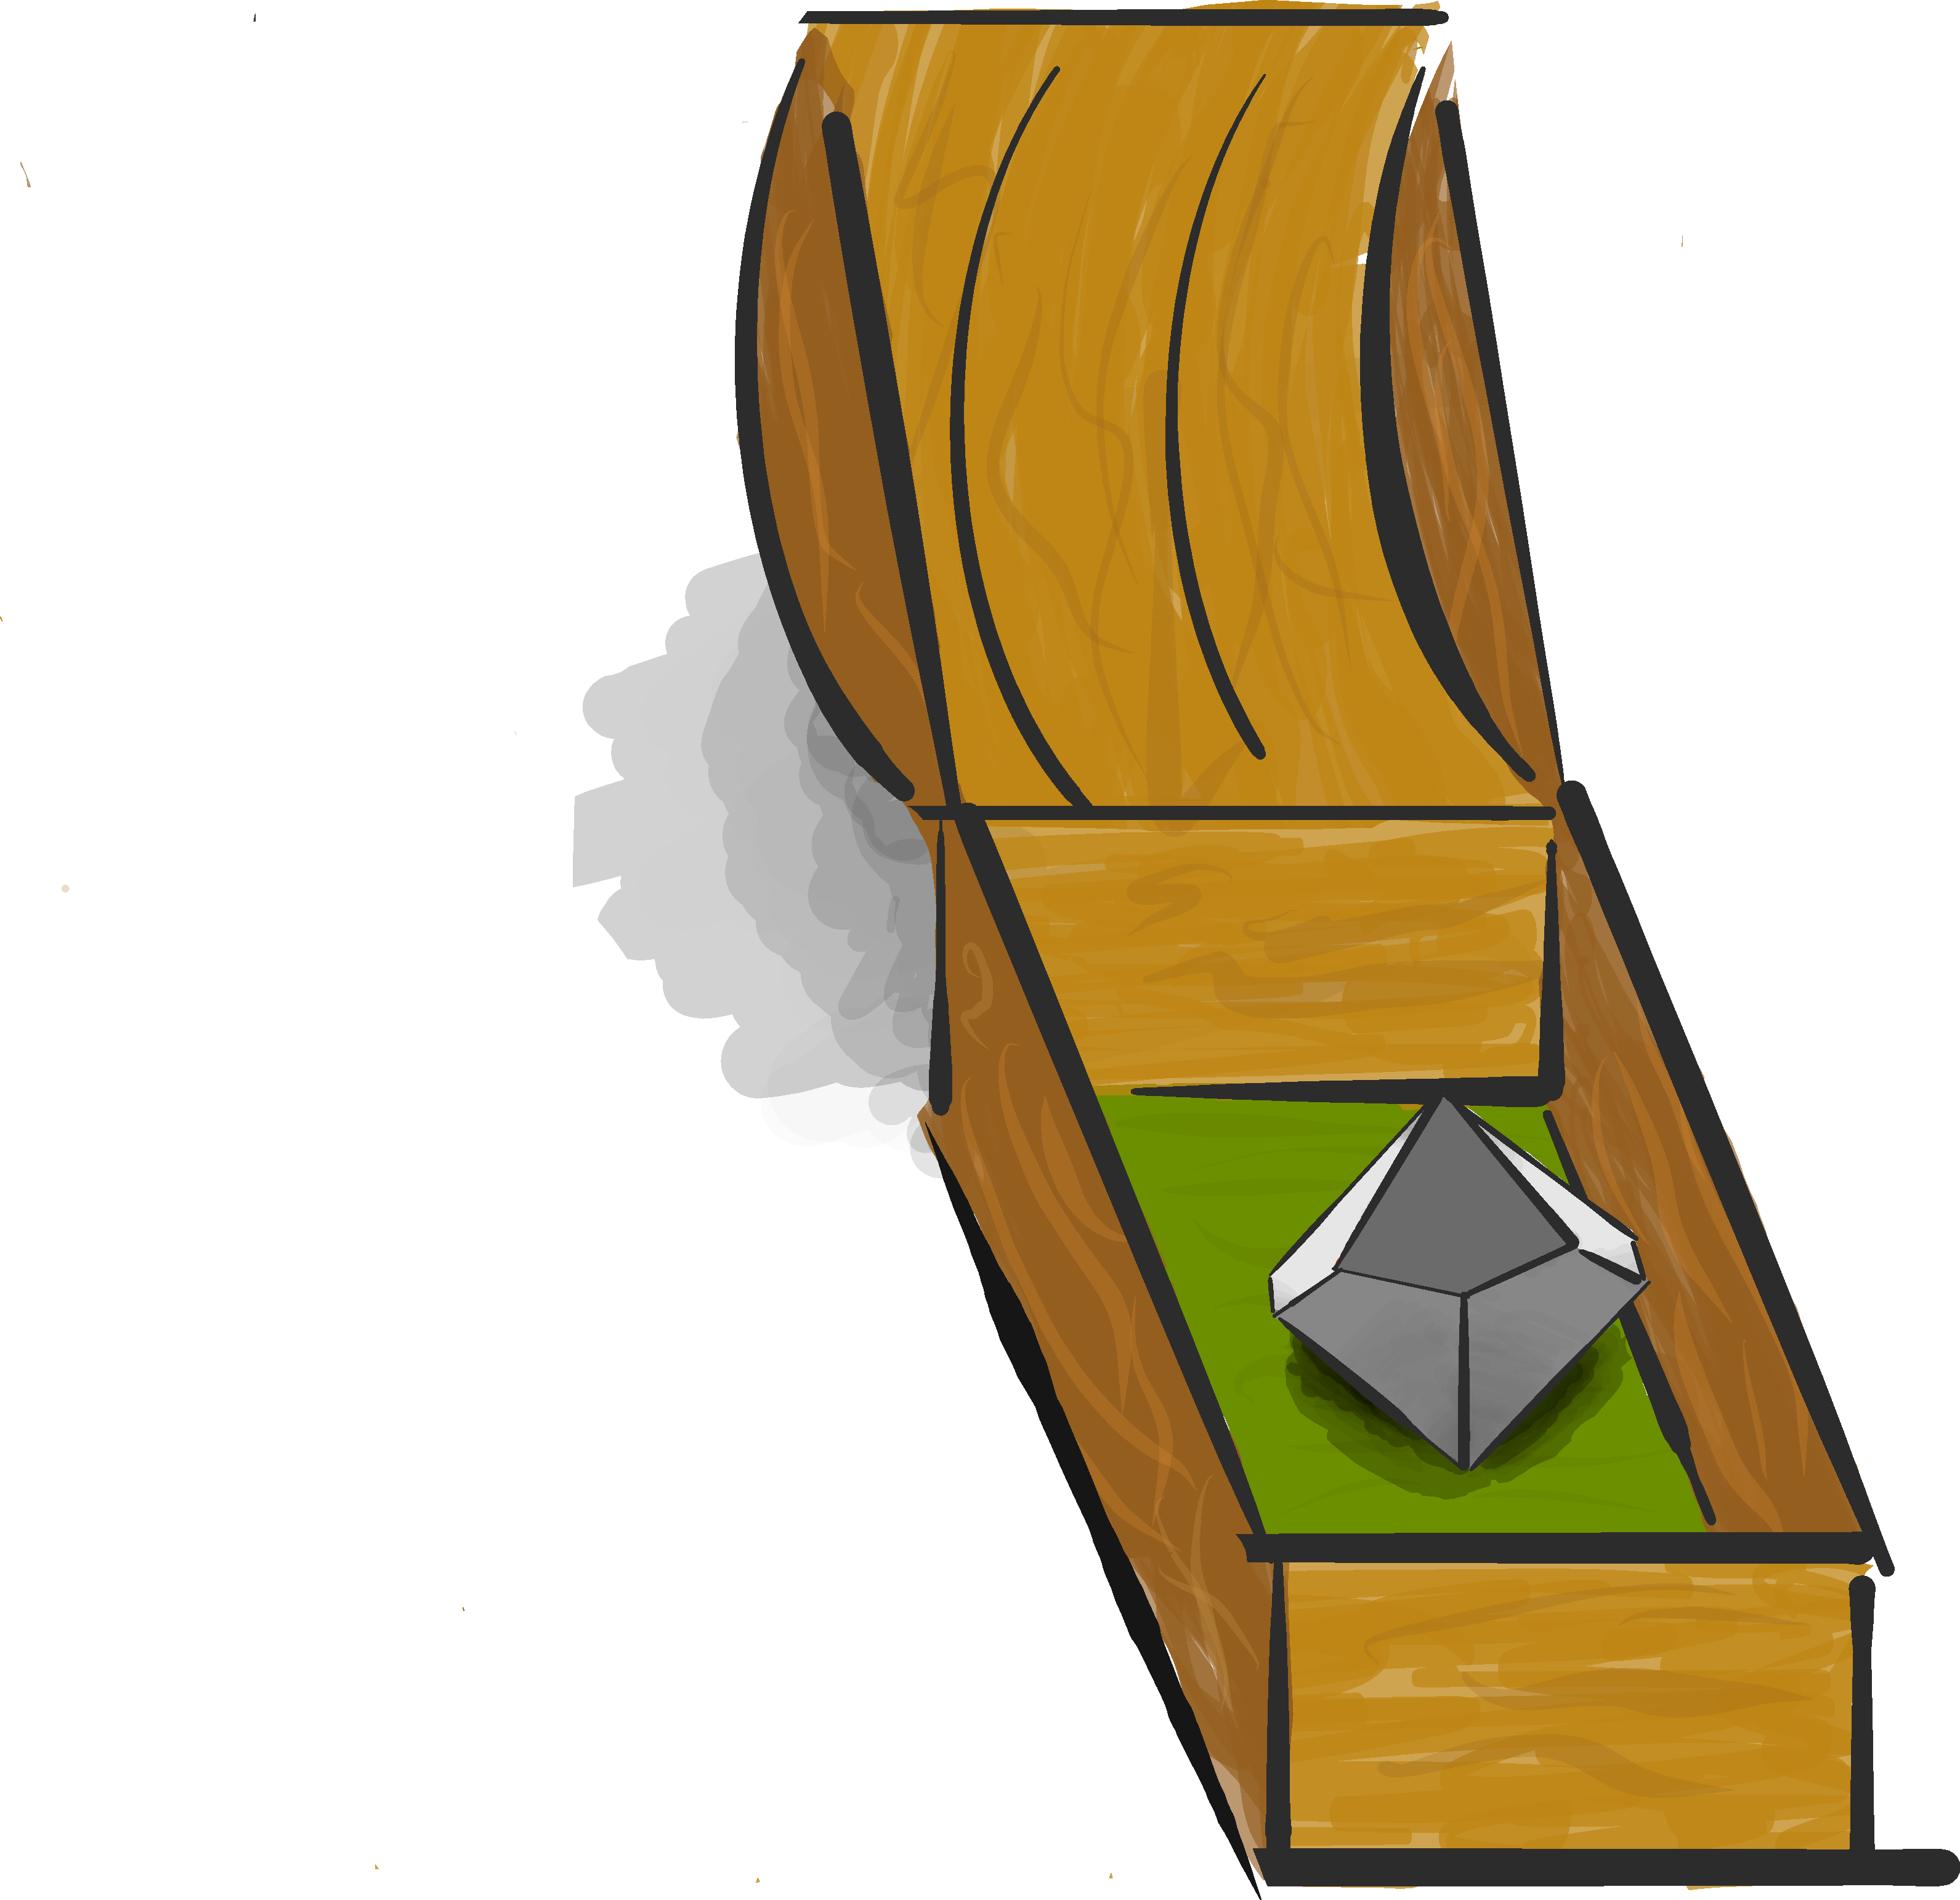
\includegraphics[width=0.3\textwidth]{img/small-box-open-die}
We close the box and give it a shake.
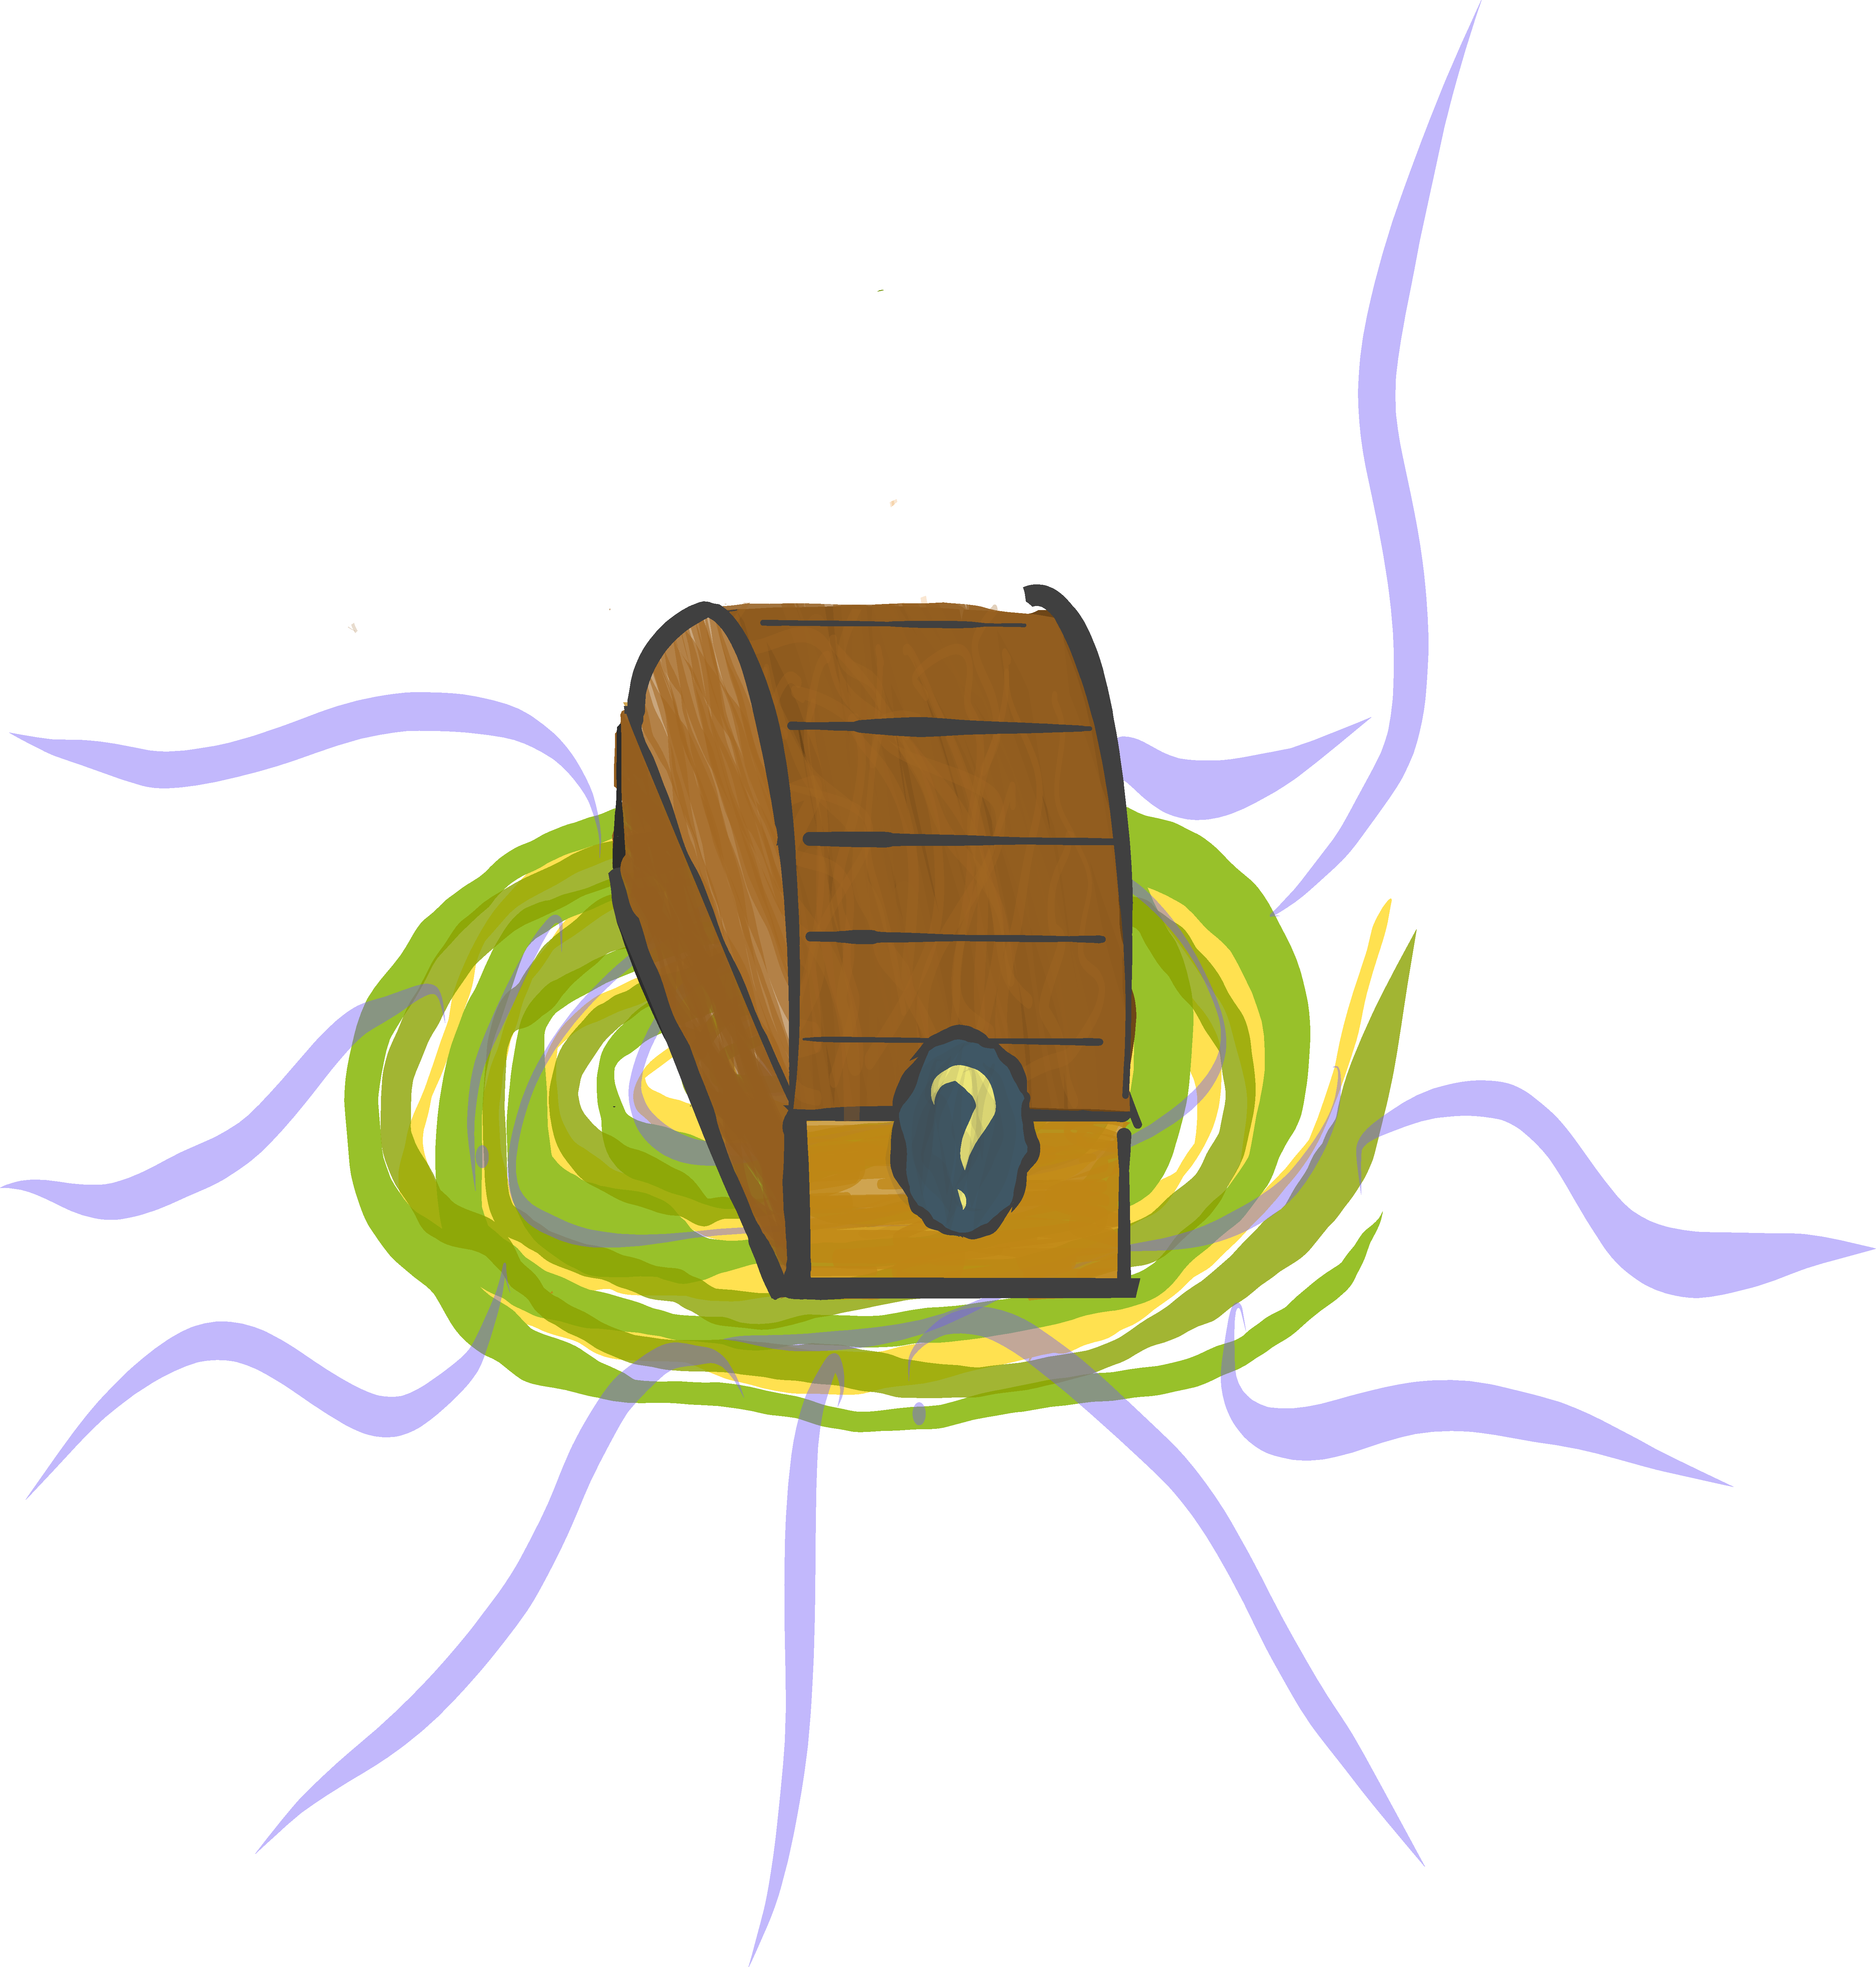
\includegraphics[width=0.3\textwidth]{img/small-box-closed-portal}
We're no longer certain which color is facing up.
As before with the coin, we're faced with uncertainty.
This raises a key question: are we more uncertain about the color facing up of the die than about the color facing up of the coin?
We can use Shannon's equation (\ref{eqn:shannon}) to answer this question.
We will calculate the entropy of the die in the box and then compare it with the entropy of the coin in the box.
Plugging and chugging with Equation \ref{eqn:snannon}, we calculate
\begin{align*}
S_{\text{die}} \approx 0.469.
\end{align*}
The die in the box has approximately 0.469 bits of entropy.
It follows that when we open the box with the die in it (and entropy returns to zero), we gain 0.469 bits of information.

So, why was more entropy associated with the coin?
Observing both the coin and the die, we recognize two outcomes: red side up or grey side up.
The difference is that for the coin, these outcomes have equal probability.
For the die, it is more likely that we will observe the grey outcome.
Thus, we can make a better guess as to what outcome we will observe on the grey die than we can for the coin.
If we always guess grey on the die, we will be correct much more often than if we always guessed grey on the coin.
So, we say that there is more uncertainty associated with the coin than with the die.
